\documentclass[10pt]{article}
\usepackage[utf8]{inputenc}
\usepackage{amsmath}
\usepackage{epsfig}
\usepackage{enumerate}
\usepackage{float}
\usepackage{listings}
\frenchspacing
\linespread{1.2}                                          %espacio entre líneas
\setlength{\parskip}{1.5ex plus 0.2ex minus 0.2ex}        %espacio entre párrafos
\setlength{\columnsep}{0.9cm}  							  %espacio entre columnas
\usepackage{indentfirst}
\usepackage{graphicx}
\usepackage{verbatim}
\usepackage{url}
\usepackage{multicol}
\usepackage{geometry}
\usepackage{fancyhdr}
\usepackage{moreverb}

\geometry{tmargin=4.5cm, lmargin=3.0cm, rmargin=2.5cm, bmargin=2.0cm}

\newcommand\R{R} %Sentencia para crear nuevos comandos.
\newenvironment{keywords}{\begin{description}\item[Keywords:]}{\end{description}}

\title{
\center{
	\textbf{ACS Community Branch}
	}
\author{Universidad Técnica Federico Santa María \\
	Computer Systems Research Group \\ \\ \\
	Tomás Staig \\ \url{tstaig@csrg.inf.utfsm.cl} \\
	Jonathan Antognini \\ \url{jantogni@csrg.inf.utfsm.cl} \\
	}
\date{Valparaíso, \today}
}

\fancyhf{}
\fancyhead[L]{ACS Community Branch}
\fancyhead[R]{\thepage}
\fancyfoot[L]{{\small Universidad Técnica Federico Santa María}}
\fancyfoot[R]{{\small Tomás Staig Jonathan Antognini}}
\pagestyle{fancy}

\begin{document}
\maketitle

\vspace{0.5cm}

\begin{center}
	\begin{abstract}
		ALMA Common Software (ACS) is a development framework that provides distributed systems functionalities. This framework was initially created to be used in the 
Atacama Large Milimiter/Submilimiter Array (ALMA) project, but due to its open source nature, there are already other projects using it. 
%but its open source property enabled other projects to be using it as well.%
Now that the development phase of ACS for ALMA is in its final stage, there is the intent of generating a more active community around it, to promote continuous 
development of the framework.
To achieve this task an initial guidelines proposal for a community branch of ACS is presented.
%An initial guidelines proposal for a community branch of ACS is presented in order to achieve the above task.%

	\end{abstract}
\end{center}

\vspace{0.4cm}

\begin{center}
\begin{keywords}
ACS, ALMA, Community, Open Source.
\end{keywords}
\end{center}

\vspace{1cm}

\thispagestyle{empty}

\newpage
\tableofcontents

\newpage
\section{Introduction}
\begin{itemize}
	\item ACS: The ALMA Common Software (ACS) provides a software infrastructure common to all partners and consists of a documented collection of common patterns 
		and of software, which implements those patterns. The heart of ACS is based on a distributed component model, with ACS components implemented as CORBA
		objects in any of the supported programmin languages. The teams responsible for the control system development use ACS Components as the basis for 
		high level control entities and for the implementation of devices, such as an antenna mount control. ACS provides common CORBA-based services such as 
		logging as well as depleyment, error and alarm management, configuration database and lifecycle management.
		\url{http://www.eso.org/~almamgr/AlmaAcs/index.html}
	\item  ALMA: The Atacama Large Millimeter Array (ALMA) is a joint project involving astronomical organizations in Europe, North America and Japan. ALMA will 
		consist of 66 antennas operating in the millimeter and sub-millimeter wavelength range, with baselines of more than 10 km. It will be located at an 
		altitude above 5000m in the Chilean Atacama desert. The ALMA Computing group is a joint group with staff scattered on 3 continents and is responsible 
		for all the control and data flow software related to ALMA, including tools ranging from support of proposal preparation to archive access of 
		automatically created images. Early in the project it was decided that an ALMA Common Software (ACS) would be developed as a way to provide a common
		software platform to all 
		partners involved in the development a common software platform. The original assumption was that some key middleware communication via CORBA and 
		the use of XML and JAVA would be part of the project. It was intended from the beginning to develop this software in an incremental way based on 
		releases, so that it would then evolve into an essential embedded part of all ALMA software applications.
		\url{http://www.almaobservatory.org/en}
	\item OpenSource: Although designed for ALMA, ACS can and is being used in other control systems and distributed software projects, since it implements proven 
		design patterns using state of the art, reliable technology. Through the use of standard constructs and components, non-ACS developers can easily 
		understand the architecture of software modules. This makes maintenance affordable even on a very large project such as ALMA. ACS is publicly 
		available under the GNU LGPL license.
		\url{http://www.gnu.org/copyleft/gpl.html}
\end{itemize}



\newpage
\section{Community}
Current Users: ACS is currently used for the following list of observatories:
\begin{itemize}
	\item The Cherenkov Telescope Array: The CTA project is an initiative to build the next generation ground-based very high energy gamma-ray instrument. It 
		will serve as an open observatory to a wide astrophysics community and will provide a deep insight into the non-thermal high-energy universe.
		\url{http://www.cta-observatory.org/}
	\item Gran Telescopio Canarias: GTC  is a 10.4m telescope with a segmented primary mirror. It is located in one of the top astronomical sites in the Northern 
		Hemisphere: the Observatorio del Roque de los Muchachos (ORM, La Palma, Canary Islands). The GTC is a Spanish initiative leaded by the Instituto de 
		Astrofísica de Canarias (IAC). The project is actively supported by the Spanish Government and the Local Government from the Canary Islands through 
		the European Funds for Regional Development (FEDER) provided by the European Union.
		\url{http://www.gtc.iac.es/en/}
	\item Sardinia Radio Telescope: The Sardinia Radio Telescope is a large, fully steerable radio telescope currently being completed near San Basilio, province 
		of Cagliari in Sardinia, Italy. It is a collaboration among the Istituto di Radioastronomia di Bologna, the Cagliari Astronomy Observatory (Cagliari) 
		and the Arcetri Astrophysical Observatory (Florence). It has been completed in 2011.
		\url{http://www.srt.inaf.it/}
	\item Telescopio Nazionale Galileo: is a 3.58m Italian telescope located on the island of San Miguel de La Palma (or, more simply, La Palma), in the Canary 
		Islands archipelago. It is one of the largest telescopes hosted by the Roque de los Muchachos Observatory, a very important observing site in the 
		northern hemisphere. It is now operated by the "Fundación Galileo Galilei, Fundación Canaria", a no-profit institution which manages the telescope 
		on behalf of INAF, the Italian National Institute of Astrophysics. The telescope saw its first light in 1998. 
		\url{http://www.tng.iac.es/}
	\item Hexapod Telescope: The Hexapod-Telescope (HPT) is a telescope located at Cerro Armazones Observatory in northern Chile. The 1.5 metres (59 in) 
		Ritchey-Chrétien reflecting telescope is notable for the design of telescope mount. Instead of the typical mounting where the telescope moves on two 
		rotating axes, the mirror end of the telescope is supported by six extensible struts, an arrangement known as a Stewart platform. This configuration 
		allows the telescope to move in all six spatial degrees of freedom and also provides strong structural integrity.
		\url{http://www.astro.ruhr-uni-bochum.de/astro/oca/hpt.html}
	\item Atacama Pathfinder EXperiment: APEX is a 12-metre diameter telescope, operating at millimetre and submillimetre wavelengths — between infrared light and 
		radio waves. Submillimetre astronomy opens a window into the cold, dusty and distant Universe, but the faint signals from space are heavily absorbed 
		by water vapour in the Earth's atmosphere. Chajnantor is an ideal location for such a telescope, as the region is one of the driest on the planet and 
		is more than 750 m higher than the observatories on Mauna Kea, and 2400 m higher than the Very Large Telescope (VLT) on Cerro Paranal. 
		\url{http://www.apex-telescope.org/}
	\item SPARTA (only partially): ESO started the development of a common flexible platform called SPARTA for Standard Platform for Adaptive optics Real Time 
		Applications. It's a real time computer and an essentially read-noise free L3 CCD60 provide an ideal cocoon to study the different behavior of the 
		two types of wave front sensors in terms of linearity, sensitivity to calibration errors, noise propagation, specific issues to pyramid or 
		Shack-Hartmann wave front sensors, etc. 
		\url{http://www.eso.org/sci/facilities/develop/ao/tecno/sparta.html}
	\item ARIES21: The ARIES21 40 m radiotelescope is a 40 m diameter fully steerable radiotelescope which operates between 2 and 110 GHz. Located 
		in Yebes, 50 km to the east of Madrid, Spain, it is in operation since 2007. It is part of the EVN (European VLBI Network) and IVS 
		(International VLBI Service). It is operated by the Observatorio Astronómico Nacional, Instituto Geográfico Nacional.
		\url{http://www.oan.es}
\end{itemize}


\newpage
\section{Community Branch}
\begin{itemize}
	\item Licenses: ACS has been developed under the LGPL, but some of the external tools, which aren't required for a basic installation use other licenses such as GPL. For this reason it is of up-most importance to determine which pieces of software, that are not under the LGPL are required, and how to distribute them without reducing the freedom of the users of ACS to distribute their software as they intend.
	\item Technical Requirements:
		\begin{itemize}
			\item Who will be able to propose:
			\begin{itemize}
				\item (1): Current Community: The current community will be the set of projects that are based on ACS and that are 
				actively working with it.
				\item (2): Potential Users: The potential users are the projects that have shown some sort of interest in using ACS.
				\item (3): Interested people: The interested people are individuals that might be willing to contribute with ACS.
			\end{itemize}
			\item How will the proposals be made:
			\begin{itemize}
				\item (1): There should be a platform for tracking requests/proposals and the work being done.
				\item (2)(3): There should be either an open side of the platform for public requests/proposal, or direct contact 
					by e-mail or similar method. 
			\end{itemize}
			\item How will the priorities be assigned: There are a lot of variables that could affect the decision to assign the priorities, making this a non-trivial problem. We need to discuss this with the community before deciding an adequate mechanism.
		\end{itemize}
	\item Participation policies
		\begin{itemize}
			\item Who will work on the requirements
			\begin{itemize}
				\item (1): Main developers: This will be the development manpower from the group in charge of maintaining ACS.
				\item (2): Current community developers: This will be the current community manpower destined to work on 
				ACS from the set of projects that are based on ACS and that are actively working with it.
				\item (3): Volunteers: This will be volunteer work done by interested people.
				\item (4): ACS patches from ALMA: This will be a back-port effort from ALMA's official repository fixes and improvements of ACS.
			\end{itemize}
			\item How will the development be done
			\begin{itemize}
				\item (1): The work is implemented and documented by the developer, along with suitable test cases and directly committed 
					to the respository.
				\item (2): The work is implemented and documented by the developer, along with suitable test cases. Validated by a main 
					developer and directly (or indirectly) committed to the respository.
				\item (3): The work is implemented by the volunteer, who shall send a patch to the main developers. The developers should 
					validate, document and add test cases to the contribution (if the volunteer didn't provide them) and, finally, 
					commit to the repository.
				\item (4): The work is implemented by ALMA developers. The main developers should obtain the patches, resolve the 								(possible) issues and document the contribution.
			\end{itemize}
			\item Tools
			\begin{itemize}
				\item Documentation: TWiki, GitHub wiki. is a flexible, powerful, and easy to use enterprise wiki, enterprise collaboration platform, 
					and web application platform. It is a Structured Wiki, typically used to run a project development space, a document 
					management system, a knowledge base, or any other groupware tool, on an intranet, extranet or the Internet. 
				\item Task Tracking: JIRA (JIRA has a free version for OpenSource projects): JIRA sits at the center of your development team, 
					connecting the people and the work being done. Track bugs and tasks, link issues to related source code, 
					plan agile development, monitor activity, report on project status, and more. 
				\item Lean Manufacturing: Kanban plugin for JIRA. GreenHopper is an add-on for JIRA that facilitates Agile project management. 
					GreenHopper leverages JIRA's flexible workflow to fit your teams Agile process and the workflow can adapt as your team evolves.
				\item Periodical builds: Jenkins. Jenkins provides an easy-to-use so-called continuous integration system, making it easier 
					for developers to integrate changes to the project, and making it easier for users to obtain a fresh build. The automated, 
					continuous build increases the productivity. Also to ensure the status of code about different supported platforms.
				\item Periodical testing: Jenkins. To see the system stability.
			\end{itemize}
		\end{itemize}
\end{itemize}






\newpage
\section{Repository}
Public repository (Given that it is an open source project).
\begin{itemize}
	\item Options comparison (between GoogleCode, GitHub, SourceForge) \\
		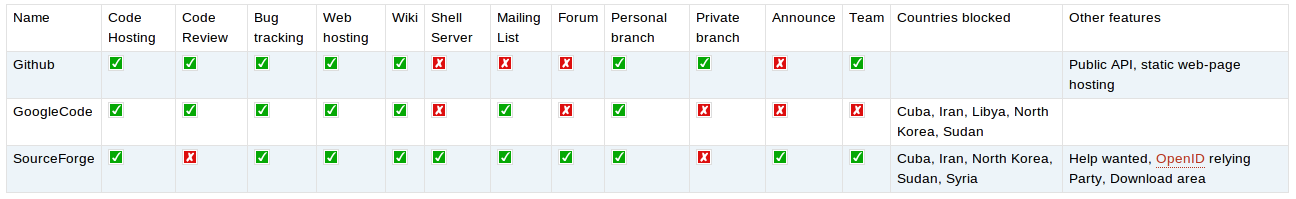
\includegraphics[width=\textwidth]{img/1.png}
	\item Available version control systems (and other features) \\
		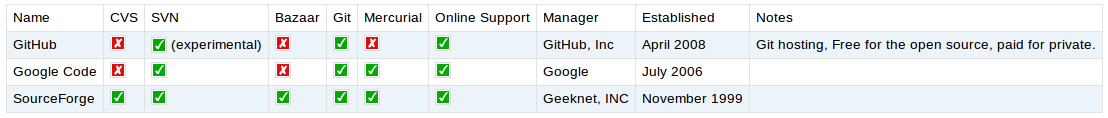
\includegraphics[width=\textwidth]{img/2.png}
	\item ACS Requirements
		\begin{itemize}
			\item Migration to the new versioning system (keeping changelogs, etc.): There are not suitable tools to convert from CVS to GIT or SVN in 
				a consistent way for large projects such as ACS. We have previously tried to convert ACS to different versioning systems obtaining 
				random loss of patches in the resulting repository. For this reason we need to analyze how this process should be done.
		\end{itemize}
	\item Veredict
		\begin{itemize}
			\item Currently GitHub does not support many version control systems, but they have the most active community (between GitHub, Source Forge 
				and Google Code), and with their Public API potential their growth. So our decision is to choose GitHub. Actually SourceForge has
				more users than Gitb Hub, but we decided according with this ratio $\frac{number\_of\_users}{years\_operatting}$.
		\end{itemize}
	\item Policies
		\begin{itemize}
			\item Branching: Reason to branch: experimental development, release maintenance.
			\item Tagging: Reason to tag: release tag.
			\item Merge: UTFSM direct, Stable Community pull request, other contributors: patch mail.
			\item Permissions
				\begin{itemize}
					\item Admin: UTFSM group.
					\item Write: UTFSM group, Stable community (pull request review).
					\item Read: anyone.	
				\end{itemize}
			\end{itemize}
\end{itemize}


\newpage
\section{Initial Maintenance and development guidelines}
\begin{itemize}
	\item First steps planning \\
		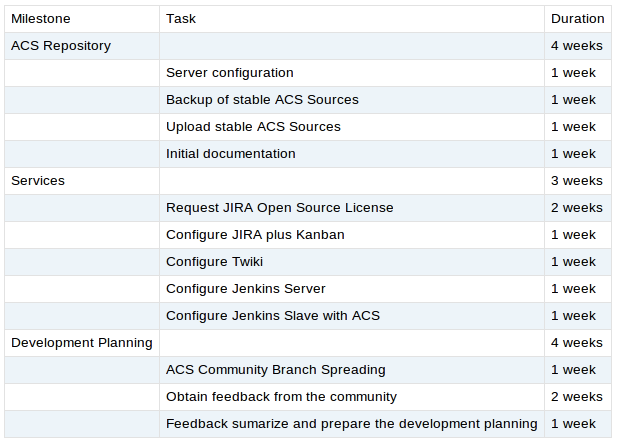
\includegraphics[width=0.65\textwidth]{img/planning.png}	
	\item Community Base Requirements
	\begin{itemize}
		\item Establish library dependencies: There is a problem in ACS to identify the dependencies for the modules/tools and external products. 
			Having this dependency tree will offer several benefits, for instance, it would facilitate the task of separating ACS into essential 
			parts, allowing to have a light version of ACS or putting it into RPM packages (or similar technologies) for easier distribution, etc. 
			It would also help in the learning curve of ACS by giving a way of navigating the different modules, knowing what are the list of 
			libraries involved in a program execution, which helps to isolate a problem to its root cause. Finally, having the list of 
			dependencies could be used to help the build process identify which sections require compilation and which can be skipped.
		\item Update external products and tools: Having the tools and external products updated could bring benefits for ACS. There are bug-fixes and 
			improvements, from which ACS can take advantage as well as support for newer platforms and build tools. Of course, along this benefits, 
			there are some costs that have to be considered, like upgrading patches created for older versions, building the newer versions, ensure 
			that new bugs that affect ACS aren't introduced, fixing API changes if they occur. To mitigate the situation where big changes occur when 
			updating the version of the products, a policy to periodically update them should be used, which should include documentation of the 
			benefits and problems that might be introduced, a set of tests if any bug is found in order to avoid regression problems. Updating all 
			the products simultaneously could be a big effort, and would be prominent to hide problems introduced between the tools. For this 
			reason, the update of the products should be done gradually or scheduled independently. In case that a new version of a tool 
			introduces unexpected new features/errors/deprecations/etc. the idea would be to patch the errors and find a workaround for unexpected 
			features/deprecations/etc. ACS maintenance for ALMA would be in charge of ESO, so the work in this branch would be independent of their
			development. The above doesn't mean that both projects could complement each other sharing features and bug-fixes.
		\item Plan to support more platforms: Having several supported platforms provides an easy way of distributing for several participants in the 
			community and increases the projects interested in using ACS by embracing their requirements. Having different supported platforms will 
			motivate the use of ACS by amateur projects, which enhances the use of a light version of ACS. Supporting more platforms doesn't come free, 
			however, as the time used in maintaining ACS increases. For this reason it is required to choose wisely how many and which platforms to 
			support. Additionally to maintenance there might be specific code required for some platforms which could produce code bloat.
		\begin{itemize}
			\item Windows
			\begin{itemize}
				\item Cygwin: There has been some work done to make ACS work with Cygwin under Windows. Currently ACS is built almost entirely and 
					behaves correctly on the core part of ACS, but some of the secondary features don't work as intended. This can be measured 
					considering the test results, which show us that around 70\% of the tests have a successful outcome.
				\item Native: There has been little work done to make ACS work natively on Windows using the Visual Studio compiler. All the External 
					Products and the Tools used by ACS were successfully built. Although ACS itself wasn't built and, for this reason, no tests 
					were made trying to run the system.
				\item Interested Projects: Windows is the operating system used by most people in the world. Therefore, providing support for this 
					system will automatically increase the opportunities to capture new projects to use ACS.
			\end{itemize}
			\item Mac: No work has been done to make ACS work under Mac, but we consider that this shouldn't be a hard task, since Mac is based on Unix 
				and provides most of the tools used by ACS.
			\begin{itemize}
				\item Interested Projects: There are several people interested in using Mac to develop with ACS and also there is a wide community 
					of amateur potential users that use Mac operating systems.
			\end{itemize}
			\item Several Linux Distributions: Currently Red Hat is the official operating system supported by ACS along with Scientific Linux which is 
				an alternative for this OS. Some work has been done to support ACS under different Linux platforms, which has led to working versions 
				of ACS under Fedora 14-16 and Ubuntu 8.04. As each operating system has its advantages and disadvantages, we shall offer alternatives 
				to the users. Considering the level of usage of the different versions of Linux by the community, we consider that the following 
				should be evaluated for support:
			\begin{itemize}
				\item Red Hat - Scientific Linux, Fedora, Ubuntu, Debian, Arch.
				\item Interested Projects: All the current projects that make use of ACS are currently using some variant of Linux, most probably Red 
					Hat or Scientific Linux. We can increase the interested projects by offering more alternatives to them.
			\end{itemize}
			\item Others (VxWorks, Solaris, HP-UX, etc.)
		\end{itemize}
		\item Plan to support more programming languages: Enhances the development of new services and tools for ACS by integrating more members of the 
			community and offering access to more libraries and integrated development environments such as .NET, Ruby on rails, etc. which offers help 
			for developing things like graphical user interfaces. On the other hand there is a lot of work to be done for implementing the infrastructure 
			for a new language to provide the services and the tools required for it.
		\item Specific GCC dependency: There is no specific dependency with GCC, although most of the code in the ACS Makefile is oriented for GCC.
		\item Compiling tools: It is possible to use different compilers either by using a compiler wrapper, or by modifying the 
			ACS Makefile. There have been some successful tests using Visual Studio compiler with the ACS Makefile for example.
		\item CUDA / OPENCL support: It should be possible to integrate ACS with parallel computing technologies.
	\end{itemize}
	\item Development
	\begin{itemize}
		\item DDS as Notification Channel: The idea is to use and extend the DDS wrapper library implemented by SPARTA project, to allow using different DDS 
			implementations, in spite of the missing standardization. SPARTA uses it for Real-Time Innovations (RTI) but keeps the option of switching it 
			in the future. ACS has extended it for OpenSplice, so far this library exists in C++ only. The task of this layer is not only to remove 
			dependencies on particular DDS implementations from the project code, but also to unify configuration of Quality of Services (QoS). 
		\item BACI Properties
		\begin{itemize}
			\item Java and Python full support
			\item Additional requirements: Depends on the feedback, could be new members, features, precision for BACI Properties, support additional 
				types, etc.
		\end{itemize}
		\item Code generator: Model Driven Architecture (MDA) software design approach is highly appraised when the project at hand has a big size. It aims
			at faster development, better communication across all levels of software, specifications and code re-usability. All these features help in
			decreasing the development time and the lines of code implemented, reducing human coding errors. 
		\item Simplify GUI creation process (Code Generation / Useful Widget Implementations / etc)
	\end{itemize}
\end{itemize}


\newpage

\thispagestyle{empty}

%\nocite{*}
%\bibliographystyle{alpha}
%\bibliography{report}

\end{document}
